\Exercise Trobeu la simetria d'una lletra "A" majúscula Arial\cite{pere_cruells_matematiques_nodate}:

%https://openaccess.uoc.edu/bitstream/10609/78485/12/Matem%C3%A0tiques%20per%20a%20multim%C3%A8dia%20I_M%C3%B2dul%207_Simetria%20i%20disseny.pdf

\begin{center}
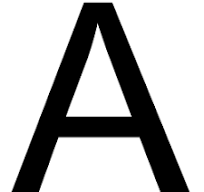
\includegraphics[scale=0.4]{A}
\end{center}

\Answer Primer identifiquem les isometries (elements de simetria que deixen la figura invariant):

\begin{itemize}
  \item La identitat $Id$.
  \item La simetria respecte l'eix verital $\sigma_v$.
  \item Cap rotació en aquest cas.
\end{itemize}

Construïm ara la taula amb les possibles composicions:

\begin{center}
\begin{tabular}{|>{\columncolor{gray}}c|c|c|}
  \hline
  \rowcolor{gray}
  $\circ$         & $Id$          & $\sigma_v$      \\\hline
  $Id$            & $Id$          & $\sigma_v$      \\\hline
  $\sigma_v$      & $\sigma_v$    & $Id$            \\\hline
\end{tabular}
\end{center}

Es tracta, doncs, d'un objecte de simetria $m$ en la notació de Hermann-Mauguin o $D_2$ en la de Schönflies.

